\documentclass{article}
\usepackage[T1]{fontenc}
\usepackage{lmodern}
\usepackage{graphicx}
\usepackage{amsmath,amssymb}
\usepackage[a4paper,margin=2cm]{geometry}
\usepackage[absolute,overlay]{textpos}
\setlength{\TPHorizModule}{1mm}
\setlength{\TPVertModule}{1mm}
\usepackage[indonesian]{babel}
\usepackage{hyperref}
\setlength{\emergencystretch}{2em}
% unit: Halaman 45

\begin{document}

% === Halaman 45 (llm) ===

\begin{itemize}
    \item Kesalahan 1-bit pada blok plainteks hanya mempengaruhi blok cipherteks yang berkoresponden saja; begitu pula pada proses dekripsi, kesalahan 1-bit pada blok cipherteks hanya mempengaruhi blok plainteks yang bersangkutan saja.
\end{itemize}

\vspace{60mm}

\begin{itemize}
    \item Karakteristik kesalahan semacam ini cocok untuk transmisi analog yang didigitisasi, seperti suara atau video, yang dalam hal ini kesalahan 1-bit dapat ditolerir, tetapi penjalaran kesalahan tidak dibolehkan.
\end{itemize}

% deskripsi: Diagram proses enkripsi (a) dan dekripsi (b) menggunakan mode operasi cipher blok yang menunjukkan bagaimana nonce dan kunci K digunakan untuk menghasilkan cipherteks C dan plainteks P.
% bbox normalisasi: [0.0080, 0.2710, 0.9640, 0.7320]
\begin{textblock*}{200.76mm}(1.68mm,80.49mm)
\noindent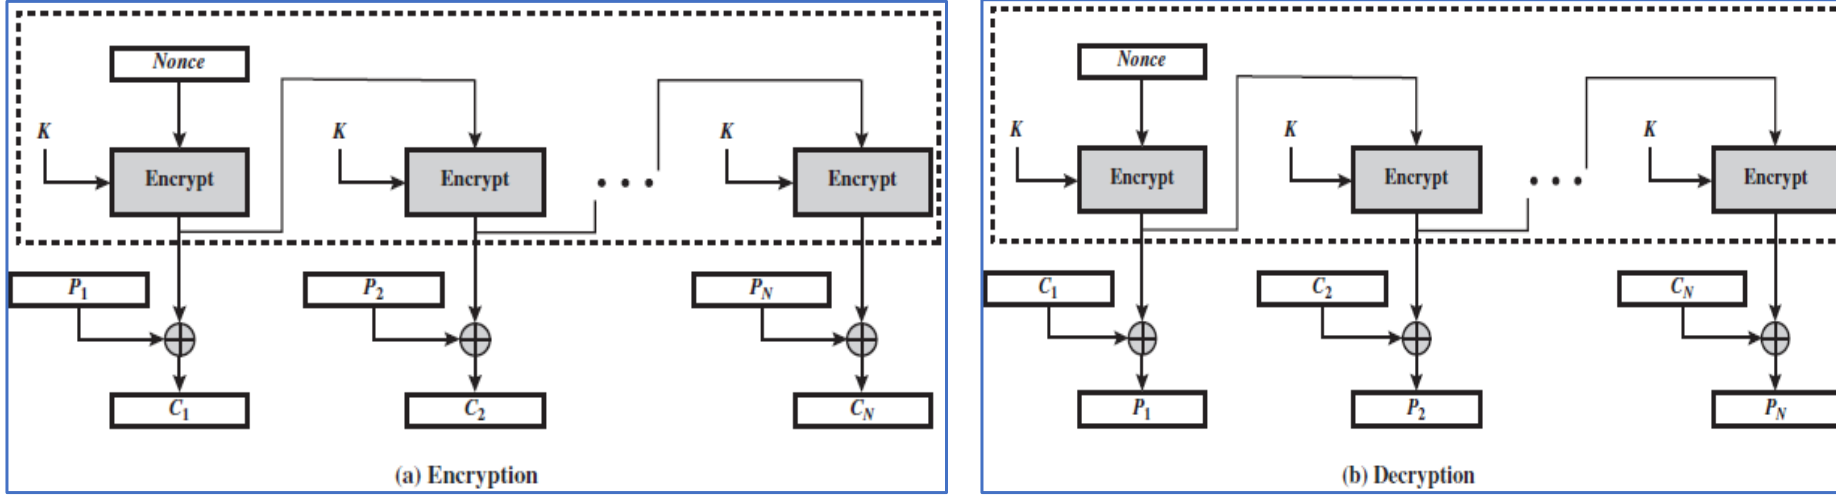
\includegraphics[width=200.76mm,height=136.92mm]{../../images/llm/page_045_img_01.png}%
\end{textblock*}

\end{document}
